
% This LaTeX was auto-generated from MATLAB code.
% To make changes, update the MATLAB code and republish this document.

\documentclass{article}
\usepackage{graphicx}
\usepackage{color}

\sloppy
\definecolor{lightgray}{gray}{0.5}
\setlength{\parindent}{0pt}

\begin{document}

    
    
\section*{Testing and Code}

\begin{par}
For testing of our code we looked at how well our functions performed relative to the native matlab functions. For the selection algorithm we only used matlab as a benchmark, as there is no exisiting function that parrellels. Please note that all the tests found here can be found in the \texttt{Mean-Value-Opt/implementation/data\_matlabazer.m} file.
\end{par} \vspace{1em}

\subsection*{Contents}

\begin{itemize}
\setlength{\itemsep}{-1ex}
   \item Data
   \item Lagrange, Variance minimization method
   \item Test Sharpe Optimization
\end{itemize}


\subsection*{Data}

\begin{par}
We start by taking a random portion of data within our dataset, as follows:
\end{par} \vspace{1em}
\begin{verbatim}[ Ret, CoRisk, stockNames, selData, data  ] = data\_selector( folders, dates(1), sectors(6) );\end{verbatim}
\begin{par}
Note that \texttt{sectors(6)} is arbitrary sector name chosen from our sectors list, and \texttt{dates(1)}, is simply the data from \texttt{2008-2009}. This function will take the data from the folder, filter it, and then store it in the \texttt{selData} variable. Then it will compute the returns, and covariance and store them in the \texttt{Ret} and \texttt{CoRisk} variables respectively. The variable \texttt{data} is simply the unfiltered dataset.
\end{par} \vspace{1em}


\subsection*{Lagrange, Variance minimization method}

\begin{par}
\textbf{Overview}:
\end{par} \vspace{1em}
\begin{par}
Building on the mathematical theory we take the covariance matrix and the returns matrix and constructs the following matrices: Note that to ensure that the program does not run for too long, we control the number of assets we wish to test. If we wanted to test \textbf{all} of the assets we would set \texttt{n = length(Ret)}.
\end{par} \vspace{1em}
\begin{verbatim}n   = 100;
M   = Ret(1:n);
S   = 2.*CoRisk(1:n,1:n);
mp  = 0.05;\end{verbatim}
\begin{verbatim}A = [ S M' ones(n,1); M 0 0 ; ones(1,n) 0 0 ];
x = [ zeros(n,1); mp; 1 ];\end{verbatim}
\begin{par}
Hence, we can obtain the solution for our wieghts as follows: \texttt{Weights = A\ensuremath{\backslash}x};
\end{par} \vspace{1em}
\begin{par}
\textbf{Testing}:
\end{par} \vspace{1em}
\begin{par}
Next we will see how our function compares to the matlab base function \texttt{quadprog}. This will surve us as a benchmark for our function. The folllowing code will compare the matlab function to us.
\end{par} \vspace{1em}
\begin{verbatim}
mp  = 0.05;
n   = length(Ret);
S   = CoRisk(1:n,1:n);
M   = Ret(1:n);

% Matlab
tic
    w = quadprog(2.*S,[],[],[],[ M ; ones(1,n)],[mp;1],...
            [],[],[],...
            optimoptions('quadprog','Algorithm','interior-point-convex','Display','off'));
    fprintf('Matlab Time:  ');
toc

% Us
tic
    WW = [ 2*S M' ones(n,1); M 0 0 ; ones(1,n) 0 0 ]\[ zeros(n,1); mp; 1 ];
    fprintf('\nUs Time:  ');
toc

% Comparison
square_root_sum_of_error_squared = sqrt(sum((WW(1:end-2)-w).^2)./n)
\end{verbatim}

        \color{lightgray} \begin{verbatim}Matlab Time:  Elapsed time is 0.009409 seconds.

Us Time:  Elapsed time is 0.000961 seconds.

square_root_sum_of_error_squared =

   1.2973e-13

\end{verbatim} \color{black}
    \begin{par}
As you can see, our function outperformed the matlab function in terms of time. This is due to the fact that the matlab function runs several tests on the matrices before actually computing the weights.
\end{par} \vspace{1em}


\subsection*{Test Sharpe Optimization}

\begin{par}
The sharpe optimization procudure we wrote, makes use of the bisection method for finding the sharpe ratio. It is stored in the \texttt{optimizeSupreme} function. For more detail, please refer to the math-section of this paper. The matlab function we chose as the benchmark is the \texttt{estimateMaxSharpeRatio} which is a part of the \texttt{Portfolio Optimization and Asset Allocation} package in matab.
\end{par} \vspace{1em}
\begin{par}
We run our comparison code as follows:
\end{par} \vspace{1em}
\begin{verbatim}
clear n M S rfr WMp mLims
clc
n       = 10;
tP      = 1:n;
M       = Ret(tP);
S       = CoRisk(tP,tP);
rfr     = RFR(1);
mLims   = 1E10;

% Matlab
tic
    p =  Portfolio('AssetMean',M,'AssetCovar',S,'RiskFreeRate',rfr,'Budget',1,'LowerBound',-mLims,'UpperBound',mLims);
    WMp = estimateMaxSharpeRatio(p);
    Matlab_Sharpe = (M*WMp-rfr)/sqrt(WMp'*S*WMp)
    fprintf('Matlab Time:  ');
toc
% Us
tic
    [ sharpe, Wp, ~, ~ ] = optimizeSupreme( M, S, rfr );
    Our_Sharpe = (M*Wp-rfr)/sqrt(Wp'*S*Wp)
    fprintf('\nUs Time:  ');
toc
\end{verbatim}

        \color{lightgray} \begin{verbatim}
Matlab_Sharpe =

    0.0963

Matlab Time:  Elapsed time is 0.808331 seconds.

Our_Sharpe =

    0.0490


Us Time:  Elapsed time is 0.010628 seconds.
\end{verbatim} \color{black}
    \begin{par}
As you can see, our function outperformed the matlab function by a great deal. As a matter of fact, it performs significally better with higher values of \texttt{n}. However, our sharpe value seems to be at first glance much lower than matlab. This is beacuse we found a \textit{parrellel} portfolio to the one of matlab. To show what we mean by that, one may simply observe the ratio between the matlab weights and our weights:
\end{par} \vspace{1em}
\begin{verbatim}
disp(WMp./Wp);
\end{verbatim}

        \color{lightgray} \begin{verbatim}   1.0e+08 *

    5.3632
    5.1647
    5.0474
    5.1848
    5.8016
    5.2656
    4.9734
    5.1739
    5.3251
    4.9616

\end{verbatim} \color{black}
    \begin{par}
Or may look at the plot of the optimization period:
\end{par} \vspace{1em}
\begin{verbatim}
figure('Name','Our Optimization');
plot(Wp'*selData(:,1:n)')
title('Our Function');
xlabel('Time');
ylabel('Value of Portfolio');
figure('Name','Matlab Optimization');
plot(WMp'*selData(:,1:n)')
title('Matlab');
xlabel('Time');
ylabel('Value of Portfolio');
\end{verbatim}

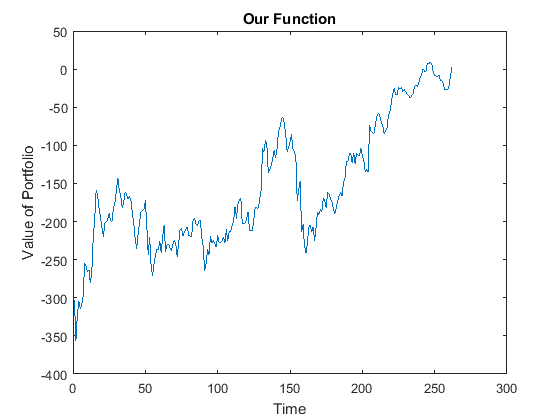
\includegraphics [width=4in]{testing_01.png}

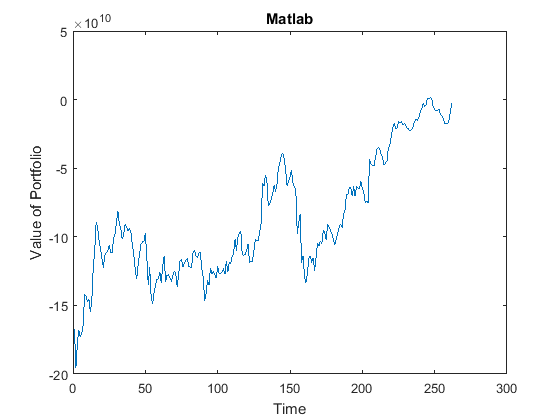
\includegraphics [width=4in]{testing_02.png}
\begin{par}
As you can see the only difference between our method and the matlab method is a multiplier. In this case the multiplier can be computed as approximately:
\end{par} \vspace{1em}
\begin{verbatim}
approximate_multiplier = mean(WMp./Wp)
WWW = approximate_multiplier.*Wp;
Our_Adjusted_Sharpe = (M*WWW-rfr)/sqrt(WWW'*S*WWW)
\end{verbatim}

        \color{lightgray} \begin{verbatim}
approximate_multiplier =

   5.2261e+08


Our_Adjusted_Sharpe =

    0.0929

\end{verbatim} \color{black}
    \begin{par}
Hence, our method compares well with matlab. As it provides us a good-enough estimate for the sharpe of the portfolio.
\end{par} \vspace{1em}



\end{document}
    
